% This LaTeX document needs to be compiled with XeLaTeX.
\documentclass[12pt]{article}
\usepackage[margin=0.8in]{geometry}
\usepackage[utf8]{inputenc}
\usepackage{graphicx}
\usepackage[export]{adjustbox}
\usepackage{amsmath}
\usepackage{amsfonts}
\usepackage{amssymb}
\usepackage[version=4]{mhchem}
\usepackage{stmaryrd}
\usepackage{bbold}
%\usepackage[fallback]{xeCJK}
\usepackage{polyglossia}
\usepackage{fontspec}
\usepackage{censor}
%\setCJKmainfont{Noto Serif CJK TC}
\graphicspath{ {../Images/} }
\usepackage{enumitem}
\usepackage{tikz}
\usepackage{amsthm}
\usepackage{tcolorbox}
\usepackage{array}
\usepackage{tabularray}
\usepackage{makecell}

\tcbuselibrary{theorems}

\definecolor{GrayCen}{HTML}{d2d2d2}
\definecolor{GrayBG}{HTML}{d9d9d9}
\definecolor{BlueDef}{HTML}{104e8b}
\definecolor{GreenProp}{HTML}{025540}
\definecolor{RedMet}{HTML}{cd5556}
\definecolor{BlackSav}{HTML}{000000}
\def\censorcolor{GrayCen}
\let\svcensorrule\censorrule
\renewcommand\censorrule[1]{%
\textcolor{\censorcolor}{\svcensorrule{#1}}}

\newtcbtheorem
  []% init options
  {definition}% name
  {Définition}% title
  {%
    colback=GrayBG,
    colframe=BlueDef,
    fonttitle=\bfseries,
  }% options
  {def}% prefix

\newtcbtheorem
  []% init options
  {proposition}% name
  {Proposition}% title
  {%
    colback=GrayBG,
    colframe=GreenProp,
    fonttitle=\bfseries,
  }% options
  {prop}% prefix

\newtcbtheorem
  []% init options
  {method}% name
  {Méthode}% title
  {%
    theorem name,
    colback=GrayBG,
    colframe=RedMet,
    fonttitle=\bfseries,
  }% options
  {met}% prefix
  
\newtcbtheorem
  []% init options
  {savoir}% name
  {Savoir-faire du chapitre}% title
  {%
    theorem name,
    colback=GrayBG,
    colframe=BlackSav,
    fonttitle=\bfseries,
  }% options
  {sav}% prefix

\newtheoremstyle{break}
  {\topsep}{\topsep}%
  {}{}%
  {\bfseries}{}%
  {\newline}{}%
\theoremstyle{break}
\newtheorem*{example}{Exemple.}
\newtheorem*{remark}{Remarque.}

\newenvironment{demo}[1][\proofname]{%
  \begin{proof}[#1]$ $\newline
}{%
  \end{proof}
}

\setmainlanguage{french}
%\setmainfont{CMU Serif}

\title{
\vspace{4em}
\centering
\tcbset{colframe=BlackSav,colback=GrayBG}
\tcbox[tikznode]{
Chapitre 4 \\Nombre dérivé et Fonction dérivée
}
}

\author{}
\date{}

\setlength\parindent{0pt}
\setlist[itemize]{noitemsep}
\setlist[enumerate]{noitemsep}

\newcolumntype{C}[1]{>{\centering\arraybackslash}m{#1}}
\newcolumntype{L}[1]{>{\raggedright\arraybackslash}m{#1}}
\newcolumntype{N}{@{}m{0pt}@{}}

\begin{document}
\maketitle

\tableofcontents

\newcommand{\hideM}[1]{\colorbox{gray!50}{\phantom{$\displaystyle #1$}}}
\newcommand{\hide}[1]{\colorbox{gray!50}{\phantom{#1}}}
%\newcommand{\hideM}[1]{#1}
%\newcommand{\hide}[1]{#1}


\newpage
\section{Nombre dérivé d'une fonction en un point}
Dans toute la suite de ce chapitre, $f: I \longrightarrow \mathbb{R}$ désigne une fonction où $I$ est un intervalle et $a \in I$. $\mathcal{C}_{f}$ désigne la courbe représentative de $f$ dans le plan muni d'un repère orthonormé $(O ; \vec{i}, \vec{j})$.

\subsection{Définition du nombre dérivé en un point}
\begin{definition}{}{}
  \begin{itemize}
    \item Pour tout $h \neq 0$ tel que $a+h \in I$, la quantité $\hideM{\dfrac{f(a+h)-f(a)}{h}}$ est appelée taux d'accroissement de $f$ entre $a$ et $a+h$.
    \item Si le taux d'accroissement tend vers un réel, lorsque $h$ tend vers 0 (avec $h \neq 0$ ), on dit que $f$ est dérivable en $a$ et on appelle \textbf{nombre dérivé} de $f$ en $a$ ce réel. On le note $f^{\prime}(a)$.\\
    On écrit :
    $$
    \hideM{\lim _{h \rightarrow 0} \frac{f(a+h)-f(a)}{h}=f^{\prime}(a).}
    $$
  \end{itemize}
\end{definition}

\begin{center}
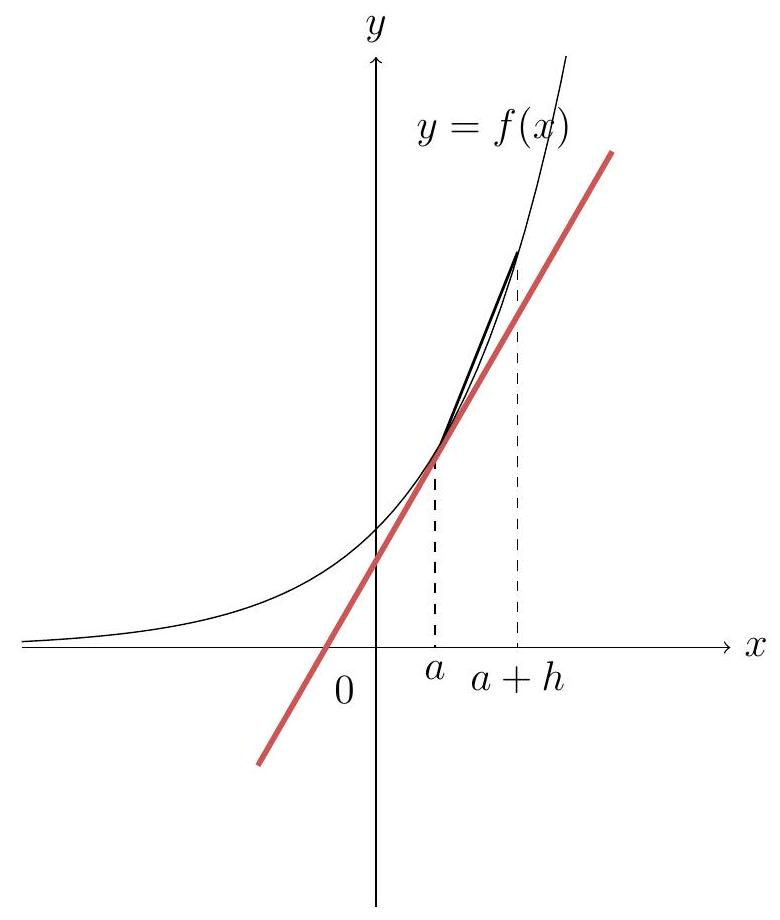
\includegraphics[max width=0.5\textwidth]{2024_12_02_3afff98cb9ed9fc6d49fg-02}
\end{center}

\begin{example}
On considère la fonction $f: x \in \mathbb{R} \longmapsto 2 x^{2}+x-2$.

Montrer que $f$ est dérivable en $a=1$ et déterminer $f^{\prime}(1)$.

\newpage
Solution :\\
Soit $h \in \mathbb{R}^{*}$,
$$
\begin{aligned}
\frac{f(1+h)-f(1)}{h} & =\frac{\left(2(1+h)^{2}+(1+h)-2\right)-\left(2 \times 1^{2}+1-2\right)}{h} \\
& =\frac{2\left(1+2 h+h^{2}\right)+(1+h)-2-1}{h} \\
& =\frac{5 h+2 h^{2}}{h} \\
& =\frac{h(5+2 h)}{h} \\
& =5+2 h \underset{h \rightarrow 0}{\longrightarrow} 5
\end{aligned}
$$

Ainsi, $f$ est dérivable en 1 et $f^{\prime}(1)=5$.
\end{example}

\begin{remark}
Attention! $f^{\prime}(a)$ n'existe pas toujours. Pour certaines fonctions, et pour certaines valeurs de $a$, il se peut que le taux d'accroissement ne tende pas vers un nombre réel (voir partie 1.3).
\end{remark}

\subsection{Tangente à une courbe en un point}
\begin{definition}{}{}
Si $f$ est dérivable en $a$, on appelle \textbf{tangente} à la courbe $\mathcal{C}_{f}$ au point d'abscisse $a$ la droite $T$ passant par le point A $\hideM{(a ; f(a))}$ et de coefficient directeur $\hideM{f^{\prime}(a)}$.
\end{definition}

\begin{remark}
Attention! Si $f$ n'est pas dérivable en $a$, il n'est \textit{a priori} pas possible de parler de la tangente à la courbe $\mathcal{C}_{f}$ au point d'abscisse $a$.
\end{remark}

\begin{proposition}{}{}
Soit $f$ une fonction dérivable en $a$.\\
L'équation de la tangente $T$ à $\mathcal{C}_{f}$ au point d'abscisse $a$ est :
$$
\hideM{y=f^{\prime}(a)(x-a)+f(a)}
$$
\end{proposition}

\begin{proof}
~\\
Soit $f$ une fonction dérivable en $a$.\\
Par définition, le coefficient directeur de la tangente $T$ à $\mathcal{C}_{f}$ au point d'abscisse $a$ est $f^{\prime}(a)$.\\
Ainsi, $T$ admet une équation de la forme $y=f^{\prime}(a) x+p$.\\
Par ailleurs, on sait que le point $A(a ; f(a))$ appartient à $T$. On obtient donc l'équation suivante :

%\begin{alignat*}{2}
\begin{equation*}
\begin{array}{rcl}
& f(a) & =f^{\prime}(a) a+p \\
\Longleftrightarrow& p & =f(a)-f^{\prime}(a) a
\end{array}
\end{equation*}
%\end{alignat*}

Finalement, l'équation de $T$ est:

$$
\begin{aligned}
y & =f^{\prime}(a) x+f(a)-f^{\prime}(a) a \\
y & =f^{\prime}(a)(x-a)+f(a)
\end{aligned}
$$
\end{proof}

\begin{example}
On considère la fonction $f: x \in \mathbb{R} \longmapsto 2 x^{2}+x-2$.\\
Déterminer l'équation de la tangente à $\mathcal{C}_{f}$ au point d'abscisse 1.

~\\Solution :\\
On a $f(1)=2 \times 1^{2}+1-2=1$.\\
Par ailleurs, on a montré que $f$ est dérivable en 1 et que $f^{\prime}(1)=5$ (voir page 2).\\
Ainsi, l'équation de la tangente est :

$$
\begin{aligned}
T: \quad & y=f^{\prime}(a)(x-a)+f(a) \\
& y=f^{\prime}(1)(x-1)+f(1) \\
& y=5 \times(x-1)+1 \\
& y=5 x-4
\end{aligned}
$$
\end{example}

\subsection{Exemples de fonctions non dérivables en un point}

\subsubsection*{Fonction racine carrée en $a=0$}
Soit $f: x \in \mathbb{R}^{+} \longmapsto \sqrt{x}$.\\
Montrons que $f$ n'est pas dérivable en $a=0$.\\
Soit $h \in \mathbb{R}_{+}^{*}$,

$$
\begin{aligned}
\frac{f(0+h)-f(0)}{h} &\ =\ \frac{\sqrt{0+h}-\sqrt{0}}{h} \\
&\ =\ \frac{\sqrt{h}}{h} \\
&\ =\ \frac{1}{\sqrt{h}}
\end{aligned}
$$

Ainsi, $\dfrac{f(0+h)-f(0)}{h} \underset{h \rightarrow 0}{\longrightarrow}+\infty$ et donc $f$ n'est pas dérivable en 0.

\begin{remark}
Géométriquement, la non-dérivabilité de la fonction racine carrée en 0 se voit au fait que la courbe admet une tangente verticale en 0.

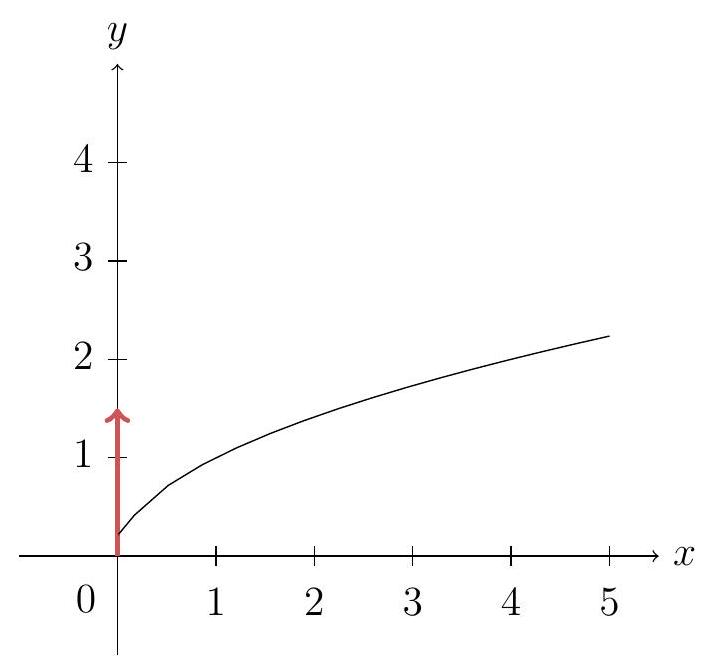
\includegraphics[max width=0.35\textwidth, center]{2024_12_02_3afff98cb9ed9fc6d49fg-04}
\begin{center}
  Fonction racine carrée
\end{center}
\end{remark}


\subsubsection*{Fonction valeur absolue en $a=0$}
Soit $f: x \in \mathbb{R} \longmapsto|x|$.\\
Montrons que $f$ n'est pas dérivable en $a=0$.\\
Soit $h \in \mathbb{R}^{*}$,

$$
\begin{aligned}
\frac{f(0+h)-f(0)}{h} & =\frac{|h|}{h} \\
& =\left\{\begin{array}{cr}
1 & \text { si } h>0 \\
-1 & \text { si } h<0
\end{array}\right.
\end{aligned}
$$

Ainsi, le taux d'accroissement $\dfrac{f(0+h)-f(0)}{h}$ ne converge pas vers une unique valeur lorsque $h$ tend vers 0. La limite n'existe pas et la fonction n'est donc pas dérivable en 0.

\begin{remark}
Géométriquement, la non-dérivabilité de la fonction valeur absolue en 0 se voit au fait que la courbe présente un «point anguleux» en 0.\\
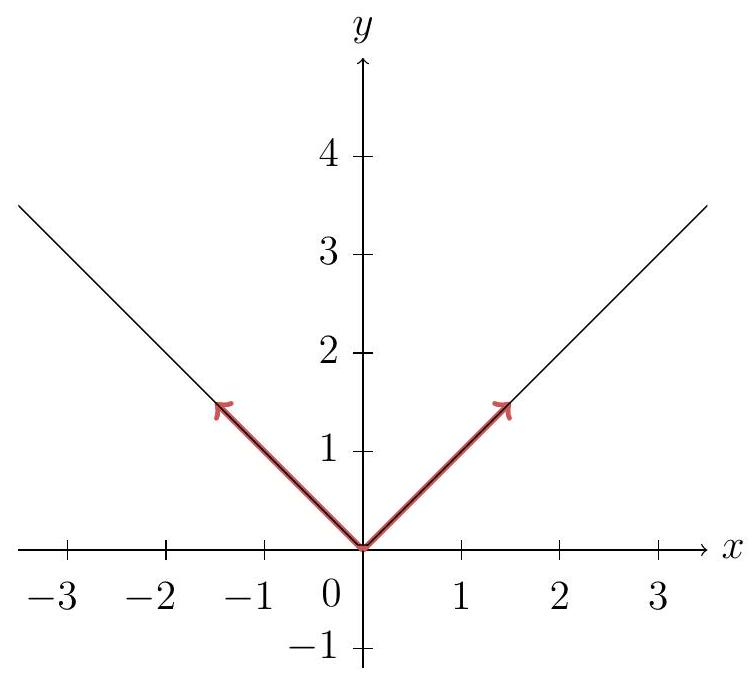
\includegraphics[max width=0.35\textwidth, center]{2024_12_02_3afff98cb9ed9fc6d49fg-05}

\begin{center}
Fonction valeur absolue
\end{center}
\end{remark}

\newpage
\section{Formules de dérivation et fonction dérivée}
\subsection{Formules de dérivation pour les fonctions de référence}

\begin{proposition}{}{}
Le tableau suivant donne les formules de dérivation pour les fonctions de référence.

\begin{center}
  \renewcommand{\arraystretch}{3.6}
  \setlength{\extrarowheight}{-3pt}
  \centering
  \begin{tabular}{|c|c|c|c|c|N}
  \hline
  Fonction & $\mathcal{D}_{f}$ & $f(x)=\ldots$ & dérivable pour $a \in \ldots$ & $f^{\prime}(a)=\ldots$ &\\
  \hline
  constante & $\mathbb{R}$ & $k$ & $\mathbb{R}$ & \hide{0} &\\
  \hline
  identité & $\mathbb{R}$ & $x$ & $\mathbb{R}$ & \hide{1} &\\
  \hline
  carrée & $\mathbb{R}$ & $x^{2}$ & $\mathbb{R}$ & $\hideM{2 a}$ &\\
  \hline
  puissance & $\mathbb{R}$ & $x^{n}$ & $\mathbb{R}$ & $\hideM{n a^{n-1}}$ &\\
  \hline
  inverse & $\mathbb{R}^{*}$ & $\frac{1}{x}$ & $\mathbb{R}^{*}$ & $\hideM{-\dfrac{1}{a^{2}}}$ &\\
  \hline
  racine carrée & $\mathbb{R}_{+}$ & $\sqrt{x}$  & $\mathbb{R}_{+}^{*}$ & $\hideM{\dfrac{1}{2 \sqrt{a}}}$ &\\
  \hline
  \end{tabular}
\end{center}
\end{proposition}

\begin{proof}
\begin{itemize}
  \item[]
  \item Soit $k \in \mathbb{R}$ et $f$ définie pour tout $x \in \mathbb{R}$ par $f(x)=k$. Soit $a \in \mathbb{R}$.

On calcule le taux d'accroissement de $f$ en $a$ :

$$
\frac{f(a+h)-f(a)}{h}=\frac{k-k}{h}=0 \underset{h \rightarrow 0}{\longrightarrow} 0
$$

Ainsi, $f$ est dérivable en $a$ et $f^{\prime}(a)=0$.

  \item Soit $f$ définie pour tout $x \in \mathbb{R}$ par $f(x)=x$. Soit $a \in \mathbb{R}$.

On calcule le taux d'accroissement de $f$ en $a$ :

$$
\frac{f(a+h)-f(a)}{h}=\frac{(a+h)-a}{h}=\frac{h}{h}=1 \underset{h \rightarrow 0}{\longrightarrow} 1
$$

Ainsi, $f$ est dérivable en $a$ et $f^{\prime}(a)=1$.
\newpage
\item Soit $f$ définie pour tout $x \in \mathbb{R}$ par $f(x)=x^{2}$. Soit $a \in \mathbb{R}$.

On calcule le taux d'accroissement de $f$ en $a$ :

$$
\begin{aligned}
\frac{f(a+h)-f(a)}{h} & =\frac{(a+h)^{2}-a^{2}}{h} \\
& =\frac{2 a h+h^{2}}{h} \\
& =\frac{h(2 a+h)}{h} \\
& =2 a+h \underset{h \rightarrow 0}{\longrightarrow} 2 a .
\end{aligned}
$$

Ainsi, $f$ est dérivable en $a$ et $f^{\prime}(a)=2 a$.

  \item On admet la formule pour la dérivée d'une fonction puissance.
  \item Soit $f$ définie pour tout $x \in \mathbb{R}^{*}$ par $f(x)=\frac{1}{x}$. Soit $a \in \mathbb{R}^{*}$.

On calcule le taux d'accroissement de $f$ en $a$ :

$$
\begin{aligned}
\frac{f(a+h)-f(a)}{h} & =\dfrac{\dfrac{1}{a+h}-\dfrac{1}{a}}{h} \\
& =\dfrac{\dfrac{a-(a+h)}{(a+h) a}}{h} \\
& =\dfrac{\dfrac{-h}{(a+h) a}}{h} \\
& =\frac{-h}{(a+h) a} \times \frac{1}{h} \\
& =-\frac{1}{(a+h) a} \underset{h \rightarrow 0}{\longrightarrow}-\frac{1}{a^{2}}
\end{aligned}
$$

Ainsi, $f$ est dérivable en $a$ et $f^{\prime}(a)=-\dfrac{1}{a^{2}}$.

  \item Soit $f$ définie pour tout $x \in \mathbb{R}_{+} \operatorname{par} f(x)=\sqrt{x}$. Soit $a \in \mathbb{R}_{+}^{*}$.

On calcule le taux d'accroissement de $f$ en $a$ :

$$
\begin{aligned}
\frac{f(a+h)-f(a)}{h} & =\frac{\sqrt{a+h}-\sqrt{a}}{h} \\
& =\frac{(\sqrt{a+h}-\sqrt{a})(\sqrt{a+h}+\sqrt{a})}{h(\sqrt{a+h}+\sqrt{a})} \\
& =\frac{(\sqrt{a+h})^{2}-(\sqrt{a})^{2}}{h(\sqrt{a+h}+\sqrt{a})} \\
& =\frac{(a+h)-a}{h(\sqrt{a+h}+\sqrt{a})} \\
& =\frac{h}{h(\sqrt{a+h}+\sqrt{a})} \\
& =\frac{1}{(\sqrt{a+h}+\sqrt{a})}\underset{h \rightarrow 0}{\longrightarrow} \frac{1}{2 \sqrt{a}}.
\end{aligned}
$$
\end{itemize}
\end{proof}

\subsection{Définition de la fonction dérivée}
\begin{definition}{}{}
Si $f$ est dérivable en tout nombre $a \in I$, on dit que $f$ est dérivable sur $I$.
\end{definition}

\begin{definition}{}{}
Si $f$ est dérivable sur $I$, la fonction qui a tout réel $x \in I$ associe $\hideM{f^{\prime}(x)}$ est appelée fonction dérivée de $f$ et elle est notée $\hideM{f^{\prime}}$.
\end{definition}

Les formules du tableau de la Proposition 2 (page 6) peuvent être reformulées de la façon suivante en l'exprimant avec les fonctions dérivées.

\begin{proposition}{}{}
\begin{center}
  \renewcommand{\arraystretch}{3.6}
  \setlength{\extrarowheight}{-3pt}
  \centering
  \begin{tabular}{|c|c|c|c|c|N}
  \hline
  Fonction & $\mathcal{D}_{f}$ & $f(x)=$ & Ensemble de dérivabilité & $f^{\prime}(x)=$ &\\
  \hline
  constante & $\mathbb{R}$ & $k$ & $\mathbb{R}$ & \hide{0} &\\
  \hline
  identité & $\mathbb{R}$ & $x$ & $\mathbb{R}$ & \hide{1} &\\
  \hline
  carrée & $\mathbb{R}$ & $x^{2}$ & $\mathbb{R}$ & $\hideM{2 x}$ &\\
  \hline
  puissance & $\mathbb{R}$ & $x^{n}$ & $\mathbb{R}$ & $\hideM{n x^{n-1}}$ &\\
  \hline
  inverse & $\mathbb{R}^{*}$ & $\frac{1}{x}$ & $\mathbb{R}^{*}$ & $\hideM{-\dfrac{1}{x^{2}}}$ &\\
  \hline
  racine carrée & $\mathbb{R}_{+}$ & $\sqrt{x}$ & $\mathbb{R}_{+}^{*}$ & $\hideM{\dfrac{1}{2 \sqrt{x}}}$ &\\
  \hline
  \end{tabular}
\end{center}
\end{proposition}

\newpage
\subsection{Dérivée et opérations sur les fonctions}
\begin{proposition}{}{}
Soient $u$ et $v$ deux fonctions dérivables sur un intervalle $I$. Soit $\lambda \in \mathbb{R}$.
\begin{center}
  \renewcommand{\arraystretch}{3.6}
  \setlength{\extrarowheight}{-3pt}
  \centering
  \begin{tabular}{|c|c|c|N}
  \hline
  Type d'opération & Fonction à dériver & Fonction dérivée \\
  %Fonction & $\mathcal{D}_{f}$ & $f(x)=$ & Ensemble de dérivabilité & $f^{\prime}(x)=$ &\\
  \hline
  \makecell{Dérivée d'une somme\\ de fonctions} & $u+v$ & $\hideM{(u+v)^{\prime}=u^{\prime}+v^{\prime}}$ &\\
  \hline
  \makecell{Dérivée du produit d'une fonction $u$ \\ par une constante $\lambda$} & $\lambda \times u$ & $\hideM{(\lambda \times u)^{\prime}=\lambda \times u^{\prime}}$ & \\
  \hline
  \makecell{Dérivée d'un produit \\ de fontions} & $u \times v$ & $\hideM{(uv)^{\prime}=u'v + uv'}$ & \\
  \hline
  \makecell{Dérivée d'un quotient \\ de fontions} & \makecell{$\dfrac{u}{v}$ avec $v(x) \neq 0$ \\ pour tout $x \in I$} & $\hideM{\left(\dfrac{u}{v}\right)'=\dfrac{u^{\prime} v-u v^{\prime}}{v^{2}}}$ & \\
  \hline
  \makecell{Dérivée de l'inverse \\ d'une fonction} & \makecell{$\frac{1}{v}$ avec $v(x) \neq 0$ \\ pour tout $x \in I$} & $\hideM{\left(\dfrac{1}{v}\right)'=-\dfrac{v'}{v^{2}}}$ & \\
  \hline
 \end{tabular}
\end{center}
\end{proposition}

\begin{remark}
Par exemple, dans la première ligne, $(u+v)^{\prime}=u^{\prime}+v^{\prime}$ est une égalité de fonctions. Cela signifie que pour tout $x \in I,(u+v)^{\prime}(x)=u^{\prime}(x)+v^{\prime}(x)$
\end{remark}

\newpage
\begin{proof}
\begin{itemize}
  \item[]
  \item Soient $u$ et $v$ deux fonctions définies et dérivables sur $I$. Soit $a \in I$. On va montrer que $u+v$ est dérivable en $a$ et que $(u+v)^{\prime}(a)=u^{\prime}(a)+v^{\prime}(a)$.\\
En fait, pour tout $h \neq 0$ :

\begin{equation*}\arraycolsep=3pt\def\arraystretch{2}
  \begin{array}{rcl}
    \dfrac{(u+v)(a+h)-(u+v)(a)}{h} & = & \dfrac{(u(a+h)+v(a+h))-(u(a)+v(a))}{h} \\
    & = &\dfrac{u(a+h)+v(a+h)-u(a)-v(a)}{h} \\
    & = &\dfrac{u(a+h)-u(a)+v(a+h)-v(a)}{h} \\
    & = &\dfrac{u(a+h)-u(a)}{h}+\dfrac{v(a+h)-v(a)}{h} \\
    & &\underset{h \rightarrow 0}{\longrightarrow} u^{\prime}(a)+v^{\prime}(a)
  \end{array}
\end{equation*}

  \item Soit $u$ une fonction définie et dérivable sur $I$ et soit $\lambda \in \mathbb{R}$. Soit $a \in I$. On va montrer que $\lambda \times u$ est dérivable en $a$ et que $(\lambda \times u)^{\prime}(a)=\lambda \times u^{\prime}(a)$. En fait, pour tout $h \neq 0$ :

\begin{equation*}\arraycolsep=3pt\def\arraystretch{2}
  \begin{array}{rcl}
    \dfrac{(u+v)(a+h)-(u+v)(a)}{h} & = & \dfrac{\lambda u(a+h)-\lambda u(a)}{h} \\
    & = & \dfrac{\lambda(u(a+h)-u(a))}{h} \\
    & = & \lambda \dfrac{u(a+h)-u(a)}{h} \\
    & & \underset{h \rightarrow 0}{\longrightarrow} \lambda u^{\prime}(a)
  \end{array}
\end{equation*}

  \item Soient $u$ et $v$ deux fonctions définies et dérivables sur $I$. Soit $a \in I$. On va montrer que $u \times v$ est dérivable en $a$ et que $(u v)^{\prime}(a)=u^{\prime}(a) v(a)+u(a) v^{\prime}(a)$.\\
  En fait, pour tout $h \neq 0$ :

\begin{equation*}\arraycolsep=3pt\def\arraystretch{2}
  \begin{array}{rcl}
    \dfrac{u v(a+h)-u v(a)}{h} & = & \dfrac{u(a+h) v(a+h)-u(a) v(a)}{h} \\
    & = & \dfrac{u(a+h) v(a+h)-u(a) v(a+h)+u(a) \times v(a+h)-u(a) v(a)}{h} \\
    & = & \dfrac{(u(a+h)-u(a)) \times v(a+h)+u(a) \times(v(a+h)-v(a))}{h} \\
    & = & \dfrac{u(a+h)-u(a)}{h} \times v(a+h)+u(a) \times \dfrac{v(a+h)-v(a)}{h} \\
    & & \underset{h \rightarrow 0}{\longrightarrow} u^{\prime}(a) \times v(a)+u(a) \times v^{\prime}(a)
  \end{array}
\end{equation*}
\newpage
  \item Soient $u$ et $v$ deux fonctions définies et dérivables sur $I$ avec, pour tout $x \in I, v(x) \neq 0$. Soit $a \in I$.\\
  On va montrer que $\dfrac{u}{v}$ est dérivable en $a$ et que $\left(\dfrac{u}{v}\right)^{\prime}(a)=\dfrac{u^{\prime}(a) \times v(a)-u(a) \times v^{\prime}(a)}{v(a)^{2}}$. En fait, pour tout $h \neq 0$ :

\begin{equation*}\arraycolsep=3pt\def\arraystretch{3.3}
  \begin{array}{rcl}
    \dfrac{\dfrac{u}{v}(a+h)-\dfrac{u}{v}(a)}{h} & = & \dfrac{\dfrac{u(a+h)}{v(a+h)}-\dfrac{u(a)}{v(a)}}{h} \\
    & = & \dfrac{\dfrac{u(a+h) v(a)-u(a) v(a+h)}{v(a+h) v(a)}}{h} \\
    & = & \dfrac{\dfrac{u(a+h) v(a)-u(a) v(a)+u(a) v(a)-u(a) v(a+h)}{v(a+h) v(a)}}{h} \\
    & = & \dfrac{\dfrac{(u(a+h)-u(a)) v(a)-u(a)(v(a+h)-v(a))}{v(a+h) v(a)}}{h} \\
    & = & \dfrac{(u(a+h)-u(a)) v(a)-u(a)(v(a+h)-v(a))}{v(a+h) v(a) \times h} \\
    %{v(a+h(a)) v(a)-u(a)(v(a+h)-v(a))} \\
    & = & \dfrac{\dfrac{(u(a+h)-u(a)) v(a)-u(a)(v(a+h)-v(a))}{h}}{v(a+h) v(a)} \\
    & = & \dfrac{\dfrac{u(a+h)-u(a)}{h}v(a)-u(a)\dfrac{v(a+h)-v(a)}{h}}{v(a+h) v(a)} \\
    & = & \dfrac{u(a+h)-u(a)}{h} v(a)-u(a) \dfrac{v(a+h)-v(a)}{h} \\
    & & \underset{h \rightarrow 0}{\longrightarrow} \dfrac{u'(a) \times v(a) - u(a) \times v'(a)}{v(a)^2}
  \end{array}
\end{equation*}

  \item Soit $v$ une fonction définie et dérivable sur $I$ avec, pour tout $x \in I, v(x) \neq 0$. Soit $a \in I$. La fonction $\dfrac{1}{v}$ est un cas particulier d'un quotient $\dfrac{u}{v}$ avec $u(x)=1$ et donc $u^{\prime}(x)=0$ Ainsi, d'après la formule de la dérivée d'un quotient :


\begin{equation*}\arraycolsep=3pt\def\arraystretch{2}
  \begin{array}{rcl}
    \left(\dfrac{1}{v}\right)^{\prime}(a) & =\dfrac{u^{\prime}(a) \times v(a)-u(a) \times v^{\prime}(a)}{v(a)^{2}} \\
    & =\dfrac{0 \times v^{\prime}(a)-1 \times v^{\prime}(a)}{v(a)^{2}} \\
    & =\dfrac{-v^{\prime}(a)}{v(a)^{2}}
  \end{array}
\end{equation*}
\end{itemize}
\end{proof}

\begin{example}
Calculer les dérivées des fonctions suivantes définies sur $\mathbb{R}$ par:

\begin{enumerate}
  \item $f(x)=x^{2}+\dfrac{1}{x}$
  \item $f(x)=5 x^{2}$
  \item $f(x)=\dfrac{x+1}{x^{2}+3}$
\end{enumerate}

Solution :
\begin{enumerate}
  \item On a $f=u+v$ avec, pour tout $x \in \mathbb{R}, u(x)=x^{2}$ et $v(x)=\dfrac{1}{x}$.
  
  On a donc, pour tout $x \in \mathbb{R}, u^{\prime}(x)=2 x$ et $v^{\prime}(x)=-\dfrac{1}{x^{2}}$. Ainsi, pour tout $x \in \mathbb{R}$ :

\begin{equation*}\arraycolsep=3pt\def\arraystretch{1.5}
  \begin{array}{rcl}
  f^{\prime}(x) & = & u^{\prime}(x)+v^{\prime}(x) \\
  & = & 2 x-\dfrac{1}{x^{2}}
  \end{array}
\end{equation*}

  \item On a $f=\lambda u$ avec, $\lambda=5$ et pour tout $x \in \mathbb{R}, u(x)=x^{2}$.

  On a donc, pour tout $x \in \mathbb{R}, u^{\prime}(x)=2 x$. Ainsi, pour tout $x \in \mathbb{R}$ :

\begin{equation*}\arraycolsep=3pt\def\arraystretch{1.2}
  \begin{array}{rcl}
  f^{\prime}(x) & = & 5 \times u^{\prime}(x) \\
  & = & 5 \times 2 x \\
  & = & 10 x
  \end{array}
\end{equation*}
  \item $f(x)=\dfrac{u(x)}{v(x)}$ avec $u(x)=x+1$ et $v(x)=x^{2}+3$ (pour tout $x \in \mathbb{R}, v(x) \neq 0$ ).

  On a, pour tout $x \in \mathbb{R}, u^{\prime}(x)=1$ et $v^{\prime}(x)=2 x$. Ainsi,

\begin{equation*}\arraycolsep=3pt\def\arraystretch{2}
  \begin{array}{rcl}
  f^{\prime}(x) & = & \dfrac{u^{\prime}(x) v(x)-u(x) v^{\prime}(x)}{v(x)^{2}} \\
  & = & \dfrac{1 \times\left(x^{2}+3\right)-(x+1) \times 2 x}{\left(x^{2}+3\right)^{2}} \\
  & = & \dfrac{x^{2}+3-2 x^{2}-2 x}{\left(x^{2}+3\right)^{2}} \\
  & = & \dfrac{-x^{2}-2 x+3}{\left(x^{2}+3\right)^{2}}
  \end{array}
\end{equation*}
\end{enumerate}
\end{example}

\subsection{Dérivée d'une fonction composée d'une fonction dérivable et d'une fonction affine}
\begin{proposition}{(admise)} 
Soit $g$ une fonction dérivable sur $I$ et soient $a$ et $b$ deux réels. Soit $J$ un intervalle tel que pour tout $x \in J, a x+b \in I$. La fonction $f$ définie sur $J$ par $f(x)=g(a x+b)$ est dérivable sur $J$ et

$$
\hideM{f^{\prime}(x)=a \times g^{\prime}(a x+b)}
$$

\end{proposition}

% $$
% x \in J \longmapsto a x+b \in I \longmapsto g(a x+b)
% $$

\begin{example}
On considère la fonction $f$ définie par $f(x)=\sqrt{3 x+1}$.
\begin{enumerate}
  \item Déterminer l'ensemble de définition de $f$.
  \item Déterminer l'ensemble de dérivabilité de $f$.
  \item Calculer $f^{\prime}(x)$ pour tout $x$ de l'ensemble de dérivabilité.
\end{enumerate}

Solution :
\begin{enumerate}
  \item Pour déterminer l'ensemble de définition, on résout l'inéquation suivante :

\begin{equation*}\arraycolsep=3pt\def\arraystretch{1.5}
  \begin{array}{rcl}
  & 3 x+1 &\geqslant 0 \\
  \Longleftrightarrow& 3 x &\geqslant-1 \\
  \Longleftrightarrow& x &\geqslant-\dfrac{1}{3}
  \end{array}
\end{equation*}

Ainsi, l'ensemble de définition de $f$ est $\mathcal{D}_{f}=\left[-\dfrac{1}{3} ;+\infty\right[$.

\item On a $f(x)=g(3 x+1)$ avec $g(x)=\sqrt{x}$.

La fonction $g$ est dérivable sur $] 0 ;+\infty[$. Ainsi, $f$ est dérivable en $x$ si $3 x+1>0$, c'est-à-dire $x>-\dfrac{1}{3}$.

Finalement, cela signifie que l'ensemble de dérivabilité de $f$ est $\left]-\dfrac{1}{3} ;+\infty\right[$.

\item En écrivant, $f(x)=g(3 x+1)$ avec $g(x)=\sqrt{x}$, on voit que $g^{\prime}(x)=\dfrac{1}{2 \sqrt{x}}$.

Ainsi, pour tout $x \in\left]-\dfrac{1}{3} ;+\infty\right[$ :

\begin{equation*}\arraycolsep=3pt\def\arraystretch{2}
  \begin{array}{rcl}
  f^{\prime}(x) & = & a \times g^{\prime}(a x+b) \\
  & = & 3 \times \dfrac{1}{2 \sqrt{3 x+1}} \\
  & = & \dfrac{3}{2 \sqrt{3 x+1}}
  \end{array}
\end{equation*}
\end{enumerate}
\end{example}

\newpage
\begin{savoir}{}{}
\begin{itemize}
  \item Déterminer un nombre dérivé par méthode graphique.
  \item Déterminer un nombre dérivé par le calcul (comme limite du taux d'accroissement ou en calculant d'abord $f^{\prime}(x)$ ).
  \item Déterminer graphiquement et par le calcul l'équation de la tangente à une courbe en un point.
  \item Calculer la dérivée d'une fonction en utilisant les formules (somme, produit, quotient, composée).
\end{itemize}
\end{savoir}

\end{document}